% !TEX root = frenetic_programmers_guide.tex

\chapter{Multi-Switch Topologies}
 \label{multiswitch_topologies}

Up until now, we've been working with a one-switch network.  Indeed, we can divide any SDN network into
one-switch subnets with a separate controller and network application for each.  We can even share
network information between these applications through a database or special network protocols.  

But this makes the SDN unncessarily complex and expensive.  By using a single controller and application
connected to a collection of switches, we gain the following:

\begin{itemize}
\item A simpler network application architecture.  Similar switches can share policy templates.
\item A cheaper infrastsucture by using one controller server (we can add redundant controllers if
fault tolerance is required).
\item A larger overall network view.  This eliminates the need for complex protocols like Spanning
Tree Protocol (STP).
\end{itemize}

The main thing in handling multi-switch networks is to avoid loops and broadcast storms.  These two 
problems can slow a network to a crawl.   

\section{A Simple Core/Edge Network}

Let's start with a fairly standard network topology.  

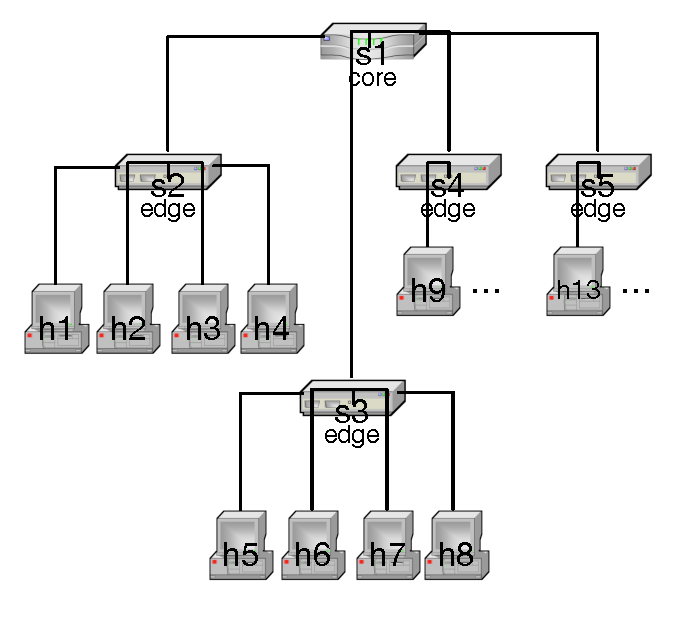
\includegraphics{switching_topo.pdf}

In this network, each of the four switches 
has four hosts of its own -- commonly one or more switches serve the hosts on a particular building floor.
These are called \emph{edge switches} because they live on the edge of the network.  Edge switches are easy to 
spot: they have end hosts connected to them.

A \emph{core switch} connects the edge switches in a bundle.  It generally doesn't have hosts
hooked up to it -- only edge switches.  

We start with the NIB from an L2 learning network and add \python{dpid} identifiers to the data
structures.

The following code is in  \codefilename{multiswitch_topologies/network_information_base.py}:

\inputminted{python}{code/multiswitch_topologies/network_information_base.py}

The core switch will have different rules than the edge switches, so we need to distinguish it
from the others.  To make things easy, we hard code the DPID of the core switch.  (We'll see 
how to obtain this information dynamically in a later section).  In a Mininet Tree topology,
the core switch always has DPID 1.  

So let's work from the edge switches inwards.  Edge switches basically learn its directly
connected hosts, like a regular L2 switch.  In fact, the NetKAT rules for the edge switch 
look like L2 rules except for the addition of \netkat{SwitchEq}.  For each learned MAC, we have a rule.

\begin{minted}{python}
Filter(SwitchEq(dpid) & EthDstEq(mac)) >> SetPort(port) 
\end{minted}

Like an L2 switch, all packets bound to/from an unlearned MAC will go the controller and get flooded
out all non-ingress ports.  The big difference, which is practically invisible in the rule, is
the packet will also go to the core switch.  That way, if the packet is bound for a host on the 
opposite side of the network, it will hop to the core switch, then to the destination switch.  

The edge switch policy is set in the application \codefilename{multiswitch_topologies/multiswitch1.py}:

\inputminted[firstline=22,lastline=40]{python}{code/multiswitch_topologies/multiswitch1.py}

And packets for unlearned MACs are handled by \python{packet_in}:

\inputminted[firstline=56,lastline=80]{python}{code/multiswitch_topologies/multiswitch1.py}

Here, we have to be a bit careful.  In a one-switch setup, we simply learn all packets coming in
on all ports.  But in a multi-switch setup, we only want to learn MACs from packets coming from
directly connected hosts.  A packet coming from a core switch comes into the \emph{uplink port}
sometimes called an \emph{internal port} because it's on an internal edge of the topology
graph.  
Such a packet represent many MACs from many hosts.  Even though those hosts may have been learned on their
ingress switches, preventing learning here, timing may cause the rules not to be installed yet.
To keep things perfectly clear, we explicitly deny learning of MAC's arriving on an internal port.
(In our first carnation, these ports are hardcoded, but we'll make it dynamic later).

Now for the core switch.  In our first incarnation, we'll take a naive approach.  We'll make it like
a repeater -- packets coming in port $p$ will be flooded out all non-$p$ ports.  This would cause problems
in a topology with loops, but our fixed topology has no loops in it and so is safe.  The edge
switch policy looks like this:

\inputminted[firstline=42,lastline=51]{python}{code/multiswitch_topologies/multiswitch1.py}

And finally because the core and edge switch policies are disjoint, we can tie them together with a 
\netkat{Union}:

\inputminted[firstline=53,lastline=54]{python}{code/multiswitch_topologies/multiswitch1.py}

We start up the Mininet topology and the Pingall pings all $16^2$ host pairs in order.  The Mininet 
topology \texttt{tree,2,4} means a tree toplogy with two levels and fanout four, meaning four
edge switches and four hosts connected to each edge switch.   

\begin{minted}{console}
vagrant@frenetic:~$ cat ~/bin/mnt4
sudo mn --topo=tree,2,4 --controller=remote --mac
vagrant@frenetic:~$ sudo mn --topo=tree,2,4 --controller=remote --mac
*** Creating network
*** Adding controller
Unable to contact the remote controller at 127.0.0.1:6633
*** Adding hosts:
h1 h2 h3 h4 h5 h6 h7 h8 h9 h10 h11 h12 h13 h14 h15 h16
*** Adding switches:
s1 s2 s3 s4 s5
*** Adding links:
(s1, s2) (s1, s3) (s1, s4) (s1, s5) (s2, h1) (s2, h2) (s2, h3) ....
*** Configuring hosts
h1 h2 h3 h4 h5 h6 h7 h8 h9 h10 h11 h12 h13 h14 h15 h16
*** Starting controller
c0
*** Starting 5 switches
s1 s2 s3 s4 s5 ...
*** Starting CLI:
mininet> pingall
*** Ping: testing ping reachability
h1 -> h2 h3 h4 h5 h6 h7 h8 h9 h10 h11 h12 h13 h14 h15 h16
h2 -> h1 h3 h4 h5 h6 h7 h8 h9 h10 h11 h12 h13 h14 h15 h16
h3 -> h1 h2 h4 h5 h6 h7 h8 h9 h10 h11 h12 h13 h14 h15 h16
h4 -> h1 h2 h3 h5 h6 h7 h8 h9 h10 h11 h12 h13 h14 h15 h16

   ... more Pings
\end{minted}

\section{Network-Wide Learning}

Out first application works, but it's pretty inefficient.  In particular:

\begin{itemize}
\item The core switch simply floods to all the switches, even when it knows where the desination switch 
and port is.  If it knows the egress switch, it should send it to that switch.  
\item Packets with an unknown destination (but a known source) get flooded out the ingress switch.  
These packets come to the controller, but they don't really need to.  They could just as well be flooded 
by a switch rule.  
\end{itemize}

So let's write some rules to handle these cases.  We need to be careful not to create loops or broadcast
storms in the process.  

First we'll do the core switch.  For every destination MAC we have learned, we know its connected to
switch $sw$ at port $p$.  Actually port $p$ doesn't matter to the core switch -- it just needs to know
which core port will get it to the egress switch $sw$.  Suppose that port is $cp$.  Then the rule will look
like:

\begin{minted}{python}
Filter(SwitchEq(core) & EthDstEq(mac)) >> SetPort(cp) 
\end{minted}

First, let's factor out the port flooding policy. 
This policy will flood all packets to all other ports on the switch.  
It will be our fallback policy for all destination MACs
we don't know.  

The following code is in \codefilename{multiswitch_topologies/multiswitch2.py}:

\inputminted[firstline=22,lastline=32]{python}{code/multiswitch_topologies/multiswitch2.py}

Next, this policy constructs the learned MAC rules.  Since there's no overlap here, a simple
\netkat{Union} can be used to combine them.  (We have factored out the \netkat{SwitchEq} filter
because we'll use it for the entire switch rule.)

\inputminted[firstline=62,lastline=70]{python}{code/multiswitch_topologies/multiswitch2.py}

Finally, the entire core switch policy puts them together.  Flooding rules and learned MAC rules have
considerable overlap -- you can imagine a packet destined for a learned MAC (which matches a learned
MAC rule) which comes in a core switch port (which matches a flooding rule).  So we use \netkat{IfThenElse}
to disambiguate them.  And here we pop on the filter for the core switch, neatly factoring it out 
of the individual rules:

\inputminted[firstline=72,lastline=80]{python}{code/multiswitch_topologies/multiswitch2.py}

OK, now for the edge switches.  We basically want to refactor the rule into the following psuedocode:

\begin{minted}{python}
if unlearned(src_mac) and not internal_port(port):  
  learn(src_mac)    # Send to controller
elif on_switch(dpid, dst_mac):
  send_directly()
else:
  flood()
\end{minted}

Like our previous application, we have to be careful not to learn MACs arriving on internal ports.
But here, since we're relying on the rules to do the flooding, not the controller, we have to 
explicitly filter out internal ports from the learning process with NetKAT predicates.

The new edge switch rule follows this psuedocode skeleton:

\inputminted[firstline=34,lastline=54]{python}{code/multiswitch_topologies/multiswitch2.py}

The remaining code stays the same.  Now doing a Ping All in Mininet is a much faster experience -- once all the
ports are learned (h1 pings each host in turn first, so that does the learning), no packets hit the controller.
Very nice!

\section{Calculating Shortest Paths}

To get to this point, we've had to effectively hard-code the network topology into the program.  It makes 
some assumptions too, for instance that the uplink port is always 5 on an edge switch.  



\section{Dynamic Toplogy Using Frenetic}


